\documentclass[11pt]{article}
\usepackage[letterpaper,margin=1in]{geometry}
\usepackage[T1]{fontenc}
\usepackage{mathptmx}
\usepackage{amsmath,amssymb}
\usepackage{graphicx}
\usepackage{booktabs}
\usepackage[font=small,labelfont=bf]{caption}
\usepackage[numbers,sort&compress]{natbib}
\usepackage{xcolor}
\usepackage{microtype}
\usepackage{authblk}
\usepackage[colorlinks=true,linkcolor=blue!50!black,citecolor=blue!50!black,urlcolor=blue!50!black]{hyperref}
\setlength{\emergencystretch}{3em}
\renewcommand{\baselinestretch}{1.12}
\newcommand{\LIO}{\texorpdfstring{LaInO$_3$}{LaInO3}}
\newcommand{\BSO}{\texorpdfstring{BaSnO$_3$}{BaSnO3}}
\newcommand{\ntot}{n_\mathrm{tot}}
\newcommand{\xmax}{x_\mathrm{max}}
\makeatletter\newcommand{\inputrows}[1]{\@@input #1 }\makeatother

\title{Mobile electrons lost at frozen gate charge: what the transport data of electrolyte-gated \LIO/\BSO\ allow}
\author{Gracen Ownby}
\affil{University of Oklahoma, Norman, Oklahoma, USA}
\date{\small 14 October 2026}

\begin{document}
\maketitle

\begin{abstract}
In the electrolyte-gated \LIO/\BSO\ two-dimensional electron gas of Lee \emph{et al.}, each gate voltage is set above the freezing point of the ionic liquid, so the positive gate charge is fixed at lower temperatures; yet between 150 and 2~K the Hall density falls by 10, 15, 26 and 40\% at 4, 5, 7 and 8~V. A Hall density below the electron density can come from subbands of unequal mobility. We test that reading against the published magnetoresistance with a self-consistent subband model and a multisubband transport calculation. At 2~K the magnetoresistance is flat to 0.1\% between 2 and 7~T, whereas independent subband channels with the required mobility differences would raise it by 1.4 (5~V) and 9.5 (7~V) percentage points. Allowing for digitization, weak localization and the suppression of the classical magnetoresistance by intersubband scattering (to no less than 0.57 of the independent-channel value in our calculations), mobility differences account for at most 13\% of the drop at 7~V and 39--75\% of it at 5~V. Coulomb scattering by the gate-induced positive charge next to the interface, which electrostatics requires, makes the upper subbands 1.3--1.9 times more mobile than the ground subband and lowers the Hall density by only 1--7\%. Most of the drop at high gate voltage is therefore a loss of mobile electrons at fixed positive charge, about $1.7\times10^{13}$~cm$^{-2}$ at 7~V. Below 50~K the conductance falls with the Hall density at nearly constant Hall mobility, by 10--27\% at 5--8~V, whereas the field-suppressible weak-localization correction read from the magnetoresistance is 2--4\%. The measured conductance also bounds how close random point charges can sit to the interface: at 8~V this bound and the electrostatic limit meet within a factor of about 1.5 for clean \BSO\ and singly charged centres, while strongly compensated \BSO\ would need their scattering reduced 3--8 times.
\end{abstract}

\section{Introduction}
The two-dimensional electron gas (2DEG) at the polar interface between \LIO\ and \BSO\ combines a polarization-induced density of a few $10^{13}$~cm$^{-2}$ with the high mobility of \BSO\ \cite{Kim2016LIO,Kim2019LIO,Aggoune2021}. Lee \emph{et al.} gated it with the ionic liquid DEME-TFSI on a 5~nm \LIO\ cap, grown by pulsed laser deposition on 110~nm of \BSO\ grown by molecular-beam epitaxy on MgO \cite{Lee2024LIO}. Each gate voltage $V_{GS}$ was applied at 220~K, where the liquid is mobile; the sample was then cooled to 2~K at constant bias and measured while warming. The liquid has its glass transition near 182~K \cite{McCann2015}, so between 2 and 150~K the ions, and with them the positive gate charge, are frozen. Their Fig.~3 gives the sheet resistance from 2 to 220~K and the Hall density $n_H$ and mobility $\mu_H$ at 2, 10, 50, 100 and 150~K for $V_{GS}=0$--8~V; their Fig.~5a gives the magnetoresistance at 2~K up to 7~T for 0, 1, 3, 5 and 7~V. At 8~V the Hall density reaches $1.08\times10^{14}$~cm$^{-2}$ at 150~K and the Hall mobility 2000~cm$^2$/Vs at 2~K. Lee \emph{et al.} note that the Hall density falls on cooling at high bias, a point they leave open, and attribute a slow rise of the resistance at low temperature to weak localization.

The fall is puzzling because the positive charge is fixed. In a companion study \cite{OwnbyMAT02} we found that the positive charge must sit within about one \LIO\ unit cell of the interface to keep electrons out of the cap at these densities. Electrons cannot disappear at fixed positive charge, so either the Hall measurement undercounts them or they leave the conducting states. The first is natural for a multisubband 2DEG: for parallel channels $n_H=(\sum_in_i\mu_i)^2/\sum_in_i\mu_i^2$ equals the electron density only when all channels have the same mobility \cite{Ziman1972}, and at $10^{14}$~cm$^{-2}$ the interface has two or three occupied subbands. The mobility differences that lower $n_H$, however, also produce a positive classical magnetoresistance. Here we use this link, with a self-consistent subband model and a multisubband transport calculation, to decide between the two possibilities, and we use the measured conductance to bound where the gate-induced charge can sit.

\section{Data}\label{sec:data}
We digitized Fig.~3b of Ref.~\cite{Lee2024LIO} (Hall density and mobility); Fig.~3a (sheet resistance) for 5--8~V, where the curves are separated; and Fig.~5a (magnetoresistance at 2~K) for 3, 5 and 7~V. The digitization is accurate to a few per cent on the logarithmic axes and to about 0.1 percentage point on the magnetoresistance. The 2~K, 8~V values ($6.49\times10^{13}$~cm$^{-2}$, 1985~cm$^2$/Vs) agree with those quoted in the text of Ref.~\cite{Lee2024LIO} to 0.7\%. The 6~V Hall markers at 2 and 10~K are hidden behind the 7~V markers, and a second reading of the 6~V series gives different values, so we do not use the 6~V Hall data.

For parallel Drude channels the conductance is $\sigma=e\,n_H\mu_H$ exactly. The resistance of Fig.~3a is 1.12--1.48 times $1/(e\,n_H\mu_H)$, a factor that grows with gate voltage and changes with temperature. Both were measured on the same Hall bar, so the difference is not geometric, and we cannot explain it. Their relative temperature dependence agrees: between 50 and 2~K the resistance rises by 9.7, 18.5 and 26.8\% at 5, 7 and 8~V in Fig.~3a and by 9.8, 23.9 and 32.0\% in the Hall data (Fig.~\ref{fig:data}b). The rise is not monotonic in gate voltage. At 6~V the resistance of Fig.~3a falls by 10\% between 50 and 2~K, and at 4~V the Hall data give a fall of 42\% with a Hall mobility rising by 86\%.

Since $n_H\le\ntot$, the largest measured Hall density, at 150~K, is a lower bound on the electron density $\ntot$; we use $\ntot=n_H(150\ \mathrm{K})$. At 2~K the Hall density is 90, 85, 74 and 60\% of it at 4, 5, 7 and 8~V (Fig.~\ref{fig:data}a), a shortfall of 0.4, 0.7, 1.9 and $4.3\times10^{13}$~cm$^{-2}$. At 2--3~V the sheet resistance is 2.5--3~k$\Omega$ ($k_Fl\approx10$), close to the metal--insulator crossover, so we concentrate on 4--8~V.

\begin{figure}[t]
\centering
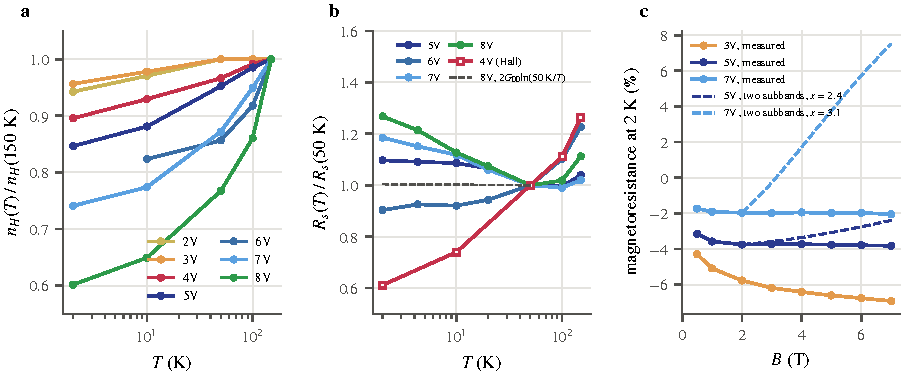
\includegraphics[width=\textwidth]{figures/fig1_data.pdf}
\caption{Data of Lee \emph{et al.} \cite{Lee2024LIO}, digitized. (a) Hall density relative to its 150~K value, with the gate charge frozen. (b) Sheet resistance relative to 50~K, from their Fig.~3a (5--8~V) and from $1/(e\,n_H\mu_H)$ (4~V). Dashed: the 8~V curve if the conductance fell by $2G_{00}\ln(50\,\mathrm{K}/T)$, about the largest that weak localization and the interaction correction give together. (c) Magnetoresistance at 2~K (their Fig.~5a), mean of $\pm B$. Dashed: the classical magnetoresistance of two independent subband channels, added to the measured value at 2~T, with the mobility ratio $x$ that reproduces the 2~K Hall density at low field (clean \BSO, measured conductance).}
\label{fig:data}
\end{figure}

\section{Model}\label{sec:model}
\emph{Subbands.} The interface is described by the self-consistent Schr\"odinger--Poisson model of Refs.~\cite{OwnbyMAT01,OwnbyMAT02}, implemented in qwkit \cite{qwkit}. Its ingredients are:
\begin{itemize}
\item a Kane-nonparabolic conduction band of \BSO\ (mass $0.19\,m_0$, nonparabolicity 0.56~eV$^{-1}$, static permittivity 20);
\item a 5~nm \LIO\ cap (offset 1.6~eV, mass $0.46\,m_0$);
\item deep acceptors in the \BSO, depleting over a width set by Fermi-level pinning;
\item a fixed interface charge that gives $5\times10^{12}$~cm$^{-2}$ without gating.
\end{itemize}
We consider strongly compensated \BSO\ ($N_A=5\times10^{19}$~cm$^{-3}$, as reported for films grown by pulsed laser deposition \cite{Kim2019LIO}) and clean \BSO\ ($10^{18}$~cm$^{-3}$). The added positive charge sits next to the interface, as Ref.~\cite{OwnbyMAT02} requires; by Gauss's law the \BSO\ side does not depend on its exact place while the cap is empty. Ten subbands enter at 2~K on a 0.5~\AA\ grid. In compensated \BSO\ the second subband is occupied only above $6.5\times10^{13}$~cm$^{-2}$ and holds 3 and 12\% of the electrons at 7 and 8~V. In clean \BSO\ the ground subband holds 84, 81, 79 and 76\% at 4, 5, 7 and 8~V. Its mean distance from the interface is 0.7--1.1~nm, against 2.0--3.0~nm for the second subband.

\emph{Scattering.} At 2~K we compute the momentum relaxation times of all occupied subbands at the Fermi level from the coupled Boltzmann equations of Siggia and Kwok \cite{SiggiaKwok1970},
\begin{equation}
1=\sum_j\left[\frac{\tau_i}{\tau^{(0)}_{ij}}-\frac{v_j}{v_i}\,\frac{\tau_j}{\tau^{(1)}_{ij}}\right],
\end{equation}
with Fermi velocities $v_i=\hslash k_i/m_i$ and nonparabolic density-of-states masses $m_i$. The matrix elements are those of point charges in the Born approximation, screened in the static random-phase approximation with the intrasubband polarizabilities of all occupied subbands \cite{SiggiaKwok1970,AFS1982}. The scatterers are:
\begin{enumerate}
\item all of the positive charge added by gating, $\ntot+N_\mathrm{dep}-\sigma_P$, as random point charges $Ze$ ($Z=1$, 2) in a plane a distance $d=1$--32~\AA\ inside the cap. They act through the cap--\BSO\ boundary, with cap permittivity $\varepsilon_\mathrm{cap}=24$, 38 or 50: the bare potential in the \BSO\ is reduced by $2\varepsilon/(\varepsilon+\varepsilon_\mathrm{cap})$, and the 2DEG's own screening acquires an image term;
\item the ionized acceptors of the depletion layer;
\item charged threading dislocations at $10^{10}$--$10^{11}$~cm$^{-2}$, typical of \BSO\ grown by molecular-beam epitaxy \cite{Paik2017}, whose bare potential acts only within a subband \cite{Jena2000};
\item interface roughness in the finite-barrier form \cite{AFS1982}, as an order-of-magnitude check.
\end{enumerate}
The relaxation times agree with an independent quadrature of the single-subband integral to $10^{-3}$, and with a direct angular solution of the coupled Boltzmann equations to $10^{-9}$. The mobilities change by less than 0.2\% between 32 and 128 angles and on a 0.25~\AA\ grid, and by 0.7--1.5\% between 10 and 14 subbands.

\emph{Magnetotransport.} For isotropic subbands the drift velocity $u_i$ of each subband obeys
\begin{equation}
m_i\sum_jG_{ij}u_j=-e(E+u_i\times B),
\end{equation}
with $G$ the relaxation matrix of the coupled Boltzmann equations. Without intersubband coupling ($G$ diagonal) this gives the classical multi-carrier Hall coefficient and magnetoresistance \cite{Ziman1972}. With coupling, intersubband scattering can suppress the magnetoresistance relative to independent channels \cite{Zaremba1992}. We compute both. Lee \emph{et al.} obtained $n_H$ from Hall resistances that were linear up to 7~T, so we compare their values with the low-field limit and with straight-line fits over 0.25--7~T.

\section{Results}
\subsection{The magnetoresistance limits mobility differences}\label{sec:mr}
At 2~K the magnetoresistance at 5 and 7~V (Fig.~\ref{fig:data}c) has a weak-localization cusp below 1~T and is then flat: between 2 and 7~T it changes by $-0.07$ and $-0.08$ percentage points. Consider two independent channels with the measured conductance, the model's $f_1$, and the mobility ratio that reproduces the 2~K Hall density at low field ($x=2.4$ at 5~V, 3.1 at 7~V). They would raise the magnetoresistance between 2 and 7~T by 1.4 and 9.5 points (dashed in Fig.~\ref{fig:data}c); with straight-line Hall fits, the required ratios and the rise are larger still. We allow the measured change plus a tolerance of 0.5 or 1.0 point, to cover digitization and a slow negative weak-localization tail. Clean \BSO\ then admits at most $x=1.73$--2.11 at 5~V and 1.33--1.50 at 7~V. These ratios permit a Hall density no lower than 0.89--0.94 (5~V) and 0.97--0.98 (7~V) of $\ntot$ (Table~\ref{tab:sum}, Fig.~\ref{fig:bounds}a). Mobility differences thus account for at most 39--75\% of the 15\% drop at 5~V, and 6--13\% of the 26\% drop at 7~V. Compensated \BSO\ has a single occupied subband at 5~V and gives no Hall deficit at all; at 7~V it allows 6--14\% of the drop.

Intersubband scattering suppresses the classical magnetoresistance relative to independent channels with the same subband mobilities \cite{Zaremba1992}. We take the Coulomb scattering of Sec.~\ref{sec:coulomb} and scale all rates to the measured conductance. At the same low-field Hall density, the coupled model then gives 0.57--1.00 times the independent-channel magnetoresistance (0.69--0.96 at 5~V, 0.57--0.96 at 7~V), so the 1.0-point tolerance covers the effect. A flat magnetoresistance could hide a large Hall deficit only if intersubband scattering were much stronger than the charged centres next to the interface produce.

The magnetoresistance also measures weak localization. The negative cusp saturates at $-3.8$\% (5~V) and $-2.0$\% (7~V), so the whole field-suppressible correction to the 2~K conductance is 2--4\%. The resistance, by contrast, rises between 50 and 2~K by 10\% at 5~V and 19--24\% at 7~V. We write the conductance change as
\begin{equation}
\sigma(50\,\mathrm{K})-\sigma(2\,\mathrm{K})=A\,G_{00}\ln 25,\qquad G_{00}=\frac{e^2}{2\pi^2\hslash},
\end{equation}
and find $A=5$--7 at 5~V, 37--63 at 7~V and 98--166 at 8~V, with $k_Fl=60$--530. Weak localization and the electron--electron interaction correction together give $A$ of a few, at most about 4--6 with several subbands and strong dephasing \cite{AltshulerAronov1980,LeeRamakrishnan1985}. Their relative size also falls as $1/k_Fl$, whereas here it grows with $k_Fl$. The resistance rise at 7--8~V is therefore not a quantum correction; at 5~V the comparison is inconclusive. Neither correction accounts for the Hall data either. Weak localization leaves the Hall coefficient unchanged, and the interaction correction changes it by twice the relative conductance change \cite{AltshulerAronov1980,LeeRamakrishnan1985}, which would make the Hall mobility rise as the conductance falls. Between 50 and 2~K, the Hall mobility instead stays within 5\% at 5--8~V while the Hall density falls by 11, 15 and 21\%.

\subsection{What the gate-induced charge does}\label{sec:coulomb}
Electrostatics places the positive charge that balances the gated electrons within a few \aa ngstr\"oms of the interface \cite{OwnbyMAT02}, and at these densities it dominates the elastic scattering. With the charge 1--6~\AA\ inside the cap ($\varepsilon_\mathrm{cap}=24$), it makes the upper subbands more mobile than the ground subband, which overlaps it most, by a factor of:
\begin{itemize}
\item 1.46--1.72 at 4~V;
\item 1.67--1.86 at 5~V;
\item 1.32--1.57 at 7~V;
\item 1.42--1.76 at 8~V.
\end{itemize}
The ratio falls towards 1, and below, as the charge moves away (Table~\ref{tab:sum}). These ratios lie within the magnetoresistance limits. Scaled to the measured conductance, they lower the Hall density to 0.959--0.990 (5~V), 0.966--0.988 (7~V) and 0.931--0.982 (8~V) of $\ntot$ (Fig.~\ref{fig:bounds}a): a few per cent, against the 15--40\% observed. Charged dislocations scatter most strongly the subbands with the smallest Fermi wavevector and lower the ratio, to 0.32--1.25 at 4~V and 1.00--1.43 at 8~V for $10^{10}$--$10^{11}$~cm$^{-2}$. Interface roughness leaves it at 1.3--1.9. In compensated \BSO\ the barely occupied second subband scatters more strongly than the ground subband ($x=0.1$--0.9). None of these static scatterers produces mobility differences large enough to explain the drop, in agreement with the magnetoresistance.

\begin{table}[t]
\centering
\small
\caption{Clean \BSO, by gate voltage. Columns: electron density $\ntot=n_H(150\,\mathrm{K})$ ($10^{13}$~cm$^{-2}$); measured $n_H/\ntot$ at 2~K; ground-subband fraction $f_1$; largest mobility ratio $x$ of the upper subbands to the ground subband allowed by the magnetoresistance at 2~K (tolerance 0.5--1.0 point), and the smallest $n_H/\ntot$ it permits (only 5 and 7~V were measured); $x$ from Coulomb scattering by the gate-induced charge at $d=1$--6~\AA\ ($Z=1$, 2; $\varepsilon_\mathrm{cap}=24$); smallest distance $d_\mathrm{min}$ (\AA) of that charge compatible with the measured conductance, from the Hall data / from Fig.~3a of Ref.~\cite{Lee2024LIO}, for $Z=1$ and $Z=2$; largest distance $\xmax$ (\AA) allowed by electrostatics at 150~K for $\varepsilon_\mathrm{cap}=24$ \cite{OwnbyMAT02}.}
\label{tab:sum}
\begin{tabular}{cccccccccc}
\toprule
$V_{GS}$ (V) & $\ntot$ & $n_H/\ntot$ & $f_1$ & $x$, MR & $n_H/\ntot$, MR & $x$, Coulomb & $d_\mathrm{min}$, $Z=1$ & $d_\mathrm{min}$, $Z=2$ & $\xmax$ \\
\midrule
\inputrows{table1.tex}
\bottomrule
\end{tabular}
\end{table}

\subsection{Where the gate-induced charge can be}\label{sec:where}
The conductance limits how strongly the gate-induced charge can scatter. Suppose other scattering only adds to it and the subband populations do not change with temperature. Then the conductivity mobility limited by that charge alone, $\mu_\sigma=\sum_i(n_i/\ntot)\mu_i$, cannot be smaller than the largest measured $\sigma/(e\ntot)$ between 2 and 150~K. From the Hall data this bound is 503, 392, 1109 and 1578~cm$^2$/Vs at 4, 5, 7 and 8~V; from the resistance of Fig.~3a it is 304, 814 and 1069~cm$^2$/Vs at 5, 7 and 8~V.

Figure~\ref{fig:bounds}b,c shows $\mu_\sigma$ against the distance of the charge, with the permittivity entering the scattering and the electrostatic limit consistently:
\begin{itemize}
\item At 4--5~V the bound is met even at 1~\AA.
\item At 7~V it requires $d\ge2.8$ or 1.6~\AA\ for $Z=1$ (Hall or Fig.~3a conductance) and $d\ge5.5$ or 4.2~\AA\ for $Z=2$, well inside the electrostatic limit of 11.6~\AA.
\item At 8~V it requires $d\ge4.9$ or 3.5~\AA\ for $Z=1$ and 7.7 or 6.0~\AA\ for $Z=2$. Electrostatics allows 4.3~\AA\ for $\varepsilon_\mathrm{cap}=24$, and 6.3 and 7.9~\AA\ for 38 and 50.
\end{itemize}
For singly charged centres, the two limits meet within a factor of 1.2 in the scattering rate at the measured cap permittivity. Doubly charged centres would need their rate reduced 1.6--2.4 times, or a cap permittivity of at least 38. Spatial correlation of the charged centres reduces their scattering in this way, strongly so at high density \cite{Efros1990,Buks1994}. These numbers come from an envelope-function model at the edge of its validity for charges a few \aa ngstr\"oms from the interface, and the electrostatic limit treats the charge as a smeared sheet, so we read them as consistent within a factor of about 1.5.

For strongly compensated \BSO, in contrast, the conductance at 8~V requires $d\ge6.5$--12.3~\AA, while electrostatics allows 1.8--2.8~\AA. The scattering rate would have to be reduced 3--8 times for $\varepsilon_\mathrm{cap}=24$, and 1.2--2.9 times for 50. Roughness with correlation lengths of 3~nm or less would by itself bring the conductivity mobility below the 7--8~V bounds; at 6--20~nm it lowers $\mu_\sigma$ by 4--19\% for 2~\AA\ steps and by 14--48\% for 4~\AA\ steps.

\begin{figure}[t]
\centering
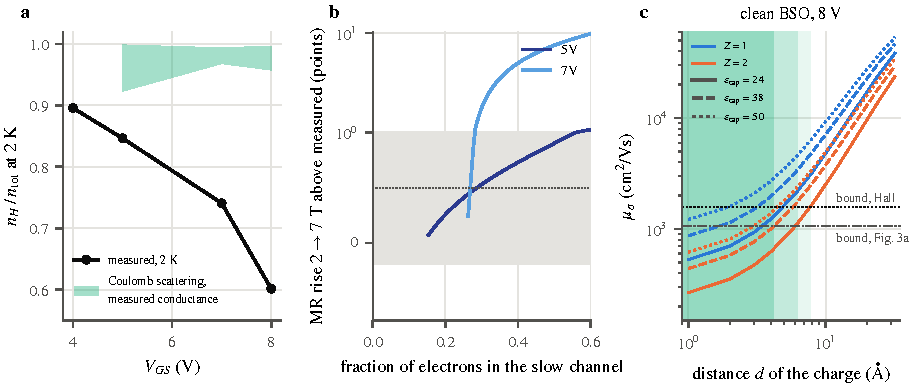
\includegraphics[width=\textwidth]{figures/fig2_bounds.pdf}
\caption{(a) Hall density relative to $\ntot$ at 2~K: measured; the smallest value that mobility differences can produce within the measured magnetoresistance (clean \BSO, tolerance 0.5 and 1.0 point); and the range produced by Coulomb scattering by the gate-induced charge at $d\le8$~\AA\ (model mobilities, $\varepsilon_\mathrm{cap}=24$). (b, c) Conductivity mobility limited by the gate-induced charge, as random point charges $Ze$ a distance $d$ inside the cap, at 7 and 8~V for clean \BSO\ and cap permittivities 24, 38 and 50. Horizontal lines: the lower bounds from the measured conductance (Hall data and Fig.~3a of Ref.~\cite{Lee2024LIO}). Shaded: distances allowed by electrostatics at 150~K \cite{OwnbyMAT02} for the three permittivities (darkest: 24).}
\label{fig:bounds}
\end{figure}

\section{Discussion}\label{sec:disc}
\emph{Electrons that leave the conducting states.} The magnetoresistance and the transport calculation agree: mobility differences between subbands explain only a small part of the Hall-density drop at 7~V, and at most part of it at 5~V. Most of the electrons that the Hall measurement misses at low temperature have therefore left the conducting states at fixed positive charge, about $1.7$--$1.8\times10^{13}$~cm$^{-2}$ of $7.3\times10^{13}$~cm$^{-2}$ at 7~V between 150 and 2~K. Below 50~K the conductance falls with the Hall density at nearly constant Hall mobility, as expected if the remaining electrons keep their mobility. Lateral inhomogeneity alone would not do this: in two dimensions a conducting film with insulating regions has the Hall coefficient of the conducting part \cite{Juretschke1956}, so regions that stop conducting raise the resistance without lowering the Hall density.

\emph{Where can they go?} In equilibrium, moving $10^{13}$~cm$^{-2}$ electrons into localized states between 50 and 2~K would need of order $10^{15}$~eV$^{-1}$cm$^{-2}$ of localized states within a few $k_BT$ of the Fermi level, at every gate voltage, which is implausible. The measurements, however, were taken while warming after cooling at constant bias \cite{Lee2024LIO}. A slow, non-equilibrium capture during cooling and a gradual release on warming would produce the observed temperature dependence. Two kinds of trap are candidates. One is localized states among the charged centres in the first \LIO\ unit cells. The other is the centres themselves: if the positive charge consists of electrochemically formed donors such as oxygen vacancies, a change of their charge state (V$_\mathrm{O}^{2+}+e\rightarrow$ V$_\mathrm{O}^{+}$) removes a mobile electron and reduces the positive charge together, without contradicting the frozen ionic charge. The cap itself remains empty: at 8~V its lowest states are 0.23~eV above the Fermi level for clean \BSO\ \cite{OwnbyMAT02}. The non-monotonic gate dependence of the resistance rise (none at 4 and 6~V) points to a process that depends on the sample or the cool-down. Comparing cooling and warming curves, or Hall data at a fixed temperature reached from above and from below, would test the non-equilibrium reading on the existing samples.

\emph{What the mobility means.} With most of the deficit due to lost carriers, the Hall mobility is close to the mobility of the remaining electrons: 1990~cm$^2$/Vs at 8~V and 2~K, for about 60\% of the gate-induced electrons. The conductance per gate-induced electron, $\sigma/(e\ntot)$, is 1200~cm$^2$/Vs at 2~K and 1580~cm$^2$/Vs at 50~K.

\emph{Limitations.}
\begin{itemize}
\item The analysis rests on digitized data from one publication. Its Supporting Information, which holds the Hall resistances, was not available to us.
\item The magnetoresistance was shown up to 7~V only, so the bound on mobility differences is direct at 5 and 7~V and inferred at 8~V.
\item The total density is taken as the 150~K Hall density, a lower bound; a larger one would increase the number of lost electrons.
\item The transport model uses the Born approximation and static screening, treats the gate-induced charge as uncorrelated point charges in a plane, and neglects exchange--correlation and phonons.
\item The roughness matrix element is first order in the step height and omits the mass-discontinuity term, so roughness is an order-of-magnitude check only.
\end{itemize}

\section{Conclusion}
In the electrolyte-gated \LIO/\BSO\ 2DEG of Lee \emph{et al.}, the Hall density at frozen gate charge falls by up to 40\% between 150 and 2~K. The published magnetoresistance, flat between 2 and 7~T, allows mobility differences between subbands to account for at most about a tenth of this fall at 7~V, and a multisubband transport calculation with the gate-induced charge next to the interface gives only a few per cent. Most of the missing electrons have therefore left the conducting states at fixed positive charge, and below 50~K the conductance falls with them. The rise of the resistance at 7--8~V is far too large for weak localization, which the magnetoresistance limits to 2--4\%. Together, the conductance and the electrostatic limit place the gate-induced charge within a few \aa ngstr\"oms of the interface for clean \BSO, consistent within a factor of about 1.5 if it consists of singly charged or correlated centres, and they argue against strongly compensated \BSO. The calculations use qwkit \cite{qwkit}.

\bibliographystyle{unsrtnat}
\bibliography{refs}
\end{document}
